\chapter{Asking Atlanta Millionaires How They Got Rich}

This chapter records a lecture whose mathematics is the mathematics of commercial mechanism rather than the mathematics of a blackboard derivation. No validated board frames survive for this lecture, so whenever we write a formula or draw a diagram, we are compressing the spoken logic of the interviews into a cleaner note form. The order matters. We begin with visible wealth, pass through a sequence of live encounters, and watch the lecture widen step by step: first to scale, then to attention, then to marketing, then to capital, and finally to the personal foundation on which durable wealth may or may not rest.

\section{Atlanta Wealth as a Field Site}

The lecture opens with a familiar but useful provocation: an extraordinary house, the promise to walk up to its owner, and the question of what kind of work could possibly support that level of visible affluence. The important thing is not the house itself. The important thing is the method. We do not begin with a theory of wealth and then hunt for illustrations; we begin with a clue, then move toward the mechanism.

The first homeowner encounter supplies the lecture's baseline quantitative anchor. We are given a local time horizon, a business count, and a best-year figure. The lecture then immediately broadens the frame. The question ``How can somebody become a millionaire in 2024?'' is raised before it is answered, and instead of resolving it abstractly the host resets the field of inquiry at the level of the city: Atlanta is introduced as a dense environment of wealthy operators, and that density justifies the case-study method that follows.

\begin{align}
T_{\text{ATL,owner}} &\approx 14\,\text{yr}, &
B_{\text{serial}} &= 6, &
Y^{\max}_{\text{serial}} &= \$15\,\mathrm{M},\\
N_{\text{ATL,millionaires}} &\approx 20{,}000. &&
\end{align}

These numbers are not yet a theory, but they do create a coordinate system. The lecture wants us to read the city as a laboratory: enough cases, enough visible outcomes, enough variation in business type, and therefore enough evidence to begin separating anecdote from mechanism.

\section{Producer, Consumer, and the Geometry of Attention}

The Lamborghini interview is the first place where the lecture ceases merely to collect stories and begins to extract a general commercial rule. The entrepreneur reports roughly fifteen years as a full-time entrepreneur, around eight years in marketing, and recent annual results a little above \$10 million. He also insists that he did not come from money; the source transcript is garbled in one short biographical stretch, but the thrust is unmistakable. The point is not inheritance. The point is construction.

\begin{align}
T_{\text{entrepreneur}} &= 15\,\text{yr}, &
T_{\text{marketing}} &= 8\,\text{yr}, &
Y^{\max}_{\text{marketing}} &> \$10\,\mathrm{M}\ \text{per year}.
\end{align}

The first conceptual distinction appears when he is asked whether he is a buyer or a seller. He answers that he is both, but only in a disciplined sense: he buys information in order to become better, and he prefers to stand on the productive side of the market. Here the lecture does something characteristic. It converts a lifestyle question into a structural one. Consumption is not denied, but it is subordinated to output.

We may write the lecture's contrast in a compressed way by letting \(P\) denote producer orientation and \(C\) denote consumer orientation. Then the operative claim is

\begin{equation}
P \succ C,
\end{equation}
not as a moral slogan but as a wealth-building posture. One may consume information, but one should do so in order to produce more effectively.

The lecture then adds the horse-blinder metaphor. This is not merely colorful language. It is an attentional model. We are meant to see that comparison, entertainment, and side-looking dissipate effort, whereas concentration on one's own lane turns attention into leverage. In these notes we may represent that mechanism schematically.

\begin{figure}[h]
\centering
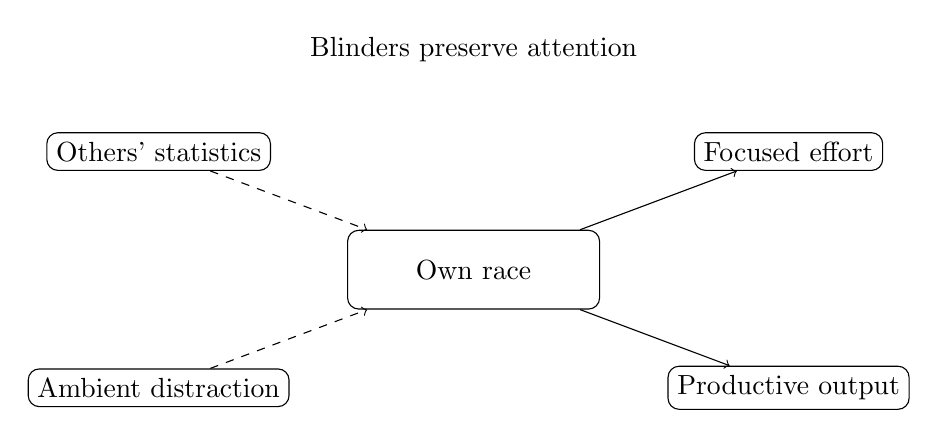
\begin{tikzpicture}
\node[draw, rounded corners] (d1) at (-4,1.5) {Others' statistics};
\node[draw, rounded corners] (d2) at (-4,-1.5) {Ambient distraction};
\node[draw, rounded corners, minimum width=3.2cm, minimum height=1cm] (c) at (0,0) {Own race};
\node[draw, rounded corners] (r1) at (4,1.5) {Focused effort};
\node[draw, rounded corners] (r2) at (4,-1.5) {Productive output};

\draw[dashed,->] (d1) -- (c);
\draw[dashed,->] (d2) -- (c);
\draw[->] (c) -- (r1);
\draw[->] (c) -- (r2);

\node at (0,2.8) {Blinders preserve attention};
\end{tikzpicture}
\caption{A transcript-based reconstruction of the lecture's blinder metaphor. Attention is treated as a scarce input into production.}
\end{figure}

If we let \(L_{\text{focus}}\) denote attention kept in one's own lane, then the lecture's implied geometry is simple: more lateral distraction means less usable energy directed toward output; stronger focus means more compounding of work in the chosen direction.

\subsection{Question \& Answer}

\paragraph{Why Do Most Businesses Fail to Scale?}

The lecture now poses a local obstacle in explicit form. If more than \(90\%\) of businesses fail to survive five years, what is the most common mistake? The answer is lack of marketing. This answer is more exact than it first appears. The lecture is not recommending a decorative layer of promotion. It is identifying visibility as a bottleneck.

\begin{equation}
p_{\text{fail by 5 yr}} > 0.9.
\end{equation}

Let \(Q_{\text{offer}}\) denote the quality of the actual offer, \(A\) the level of market awareness, and \(F\) the effective failure risk. Then the lecture's claim can be rendered as

\begin{equation}
Q_{\text{offer}} + A_{\text{low}} \Rightarrow F_{\text{high}}.
\end{equation}

The logic is short and important enough to write as a derivation.

\begin{enumerate}
\item A business may be excellent at the level of product or service.
\item If awareness \(A\) is low, the market does not know that excellence exists.
\item If the market does not know the business exists, scale stalls.
\item Repeated invisibility raises the probability of failure.
\item Therefore marketing belongs to the survival structure of the business, not to its cosmetic surface.
\end{enumerate}

To make the same point a little more explicitly, we may introduce a schematic awareness update rule. Let \(m_t\) denote marketing effort or marketing spend at stage \(t\). Then

\begin{equation}
A_T = A_0 + \sum_{t=0}^{T-1} m_t.
\end{equation}

If \(A_0\) is small and the sequence \(m_t\) is neglected, awareness never compounds. The lecture's commercial monotonicity claim may then be written

\begin{equation}
A_{\uparrow} \Rightarrow \Pr(\text{scale})_{\uparrow}.
\end{equation}

This is the first fully worked mechanism in the lecture. Good work alone is not sufficient. Good work must become legible to the market.

\section{Advice, Recoverability, and the Handling of Ambition}

Once the lecture has extracted a mechanism of market failure, it pivots toward the handling of ambition itself. The host asks whether, after losing a great deal, the entrepreneur could make it all back. The answer is yes, and the reason given is notable: he now has the mindset and the skill set. This is an early clue that the lecture is quietly building toward a deeper ordering relation that will only be stated explicitly later.

The same interview then asks for advice to a twenty-year-old self starting from zero. Here the portable maxim emerges. The biggest way to kill a big dream, he says, is to introduce it to a small mind. The lecture is no longer speaking only about markets. It is speaking about the filtration of counsel. Family may love us, but loving us is not the same as having built the thing we want to build. A coworker may be sincere, but sincerity is not expertise in entrepreneurship. The lecture therefore imposes a severe selection rule on advice: if we want to learn how to become what we are not yet, we should learn from those who already inhabit that level.

The host's recap is significant. He does not merely thank the speaker and move on. He restates the trajectory: from being broke to running an eight-figure marketing agency doing more than \$10 million in recent years. Then he extracts the line that the lecture wants us to carry forward. That recap tells us what the case was for. It was not just biography; it was an answer to the question of how ambition should be protected while it is still vulnerable.

\section{Capital, Timing, and the Real-Estate Developer's View of Scale}

The real-estate developer widens the frame. The first question is almost embarrassingly practical: does one need money to begin in real estate? The answer is yes. Real estate is expensive. This correction matters. The lecture refuses to force every field into the same low-barrier narrative. Some sectors are structurally capital-intensive.

We then receive the developer's own scale marker: a long career in commercial real-estate development and a best year of \$100 million. When asked how one scales from eight to nine figures, his answer is not simply hustle, discipline, or branding. His answer is timing. This is one of the lecture's most useful deflations. It admits circumstance, cycle, and luck into the mechanism of scale.

\begin{align}
T_{\text{RE}} &= 25\,\text{yr}, &
Y^{\max}_{\text{RE}} &= \$100\,\mathrm{M}, &
a_{\text{RE}} &\approx 56.
\end{align}

The conversation then moves into a more reflective register. The developer says that people with a billion dollars are not necessarily as smart as others imagine; many people get lucky. He then introduces a distinction that deserves to be preserved exactly.

\begin{definition}
Beliefs are what one thinks is true. Values are what one thinks is important.
\end{definition}

\begin{equation}
Bel = \text{what one thinks is true}, \qquad
Val = \text{what one thinks is important}.
\end{equation}

The point here is that capital judgment is not reducible to factual knowledge. It also requires a ranking of importance. That prepares the lecture's next move, which concerns raising money. The developer's claim is that there is more money in the world looking for good business plans than there are genuinely good business plans.

\begin{equation}
K_{\text{available capital}} > G_{\text{good business plans}}.
\end{equation}

This inequality is qualitative, not statistical, but its content is strong. The bottleneck in a mature capital market is not money in the abstract; it is the scarcity of plans that survive scrutiny. The lecture describes that scrutiny in ordinary commercial terms: margins, cost structure, path to growth, and a return legible to the investor. If we let \(R\) denote the return story that can be defended to a capital provider, then the screening chain may be written as

\begin{equation}
G_{\text{plan}} \Rightarrow \text{coherent margins} \Rightarrow \text{coherent growth path} \Rightarrow R_{\text{credible}}.
\end{equation}

This is not a board proof, but it is a clear derivational sequence. The plan is screened for intelligibility, not for beauty.

The same interview now turns one more time, and the turn matters. The host asks not about money but about happiness. The developer jokes about the exact age at which he became a millionaire, then dismisses the question as unimportant. He says he has been happy for decades, and that happiness mattered more than the bookkeeping threshold of millionaire status. The rest of the answer explains why: he had learned to manage resources in the restaurant world, discovered that those skills could transfer to development, and found that the work suited him. In other words, the lecture shifts from accumulation to fit.

That shift should not be lost, because it supplies the host's later recap: there is abundant capital in the world, but it still must be met by an idea that others can believe in, and by a worker whose skill and temperament actually match the field.

\section{From Rock Bottom to Foundation}

The lecture now circles back to the mansion teaser and executes the full interview promised at the beginning. The homeowner again identifies himself in substance as a serial entrepreneur, reports six businesses, and repeats the \$15 million peak year. But the conversation does not simply recycle the opening. It goes further. The host asks whether he is a buyer or a seller, and this time the answer is sharper: he is a seller.

This answer is then amplified by the familiar gold-rush heuristic. More people, he says, got rich during the gold rush by selling shovels than by searching for gold. The point is not historical precision. The point is market position. One profits not only by joining the scramble, but by selling into the scramble.

\begin{equation}
\Pr(\text{rich}\mid \text{sell shovels}) >
\Pr(\text{rich}\mid \text{look for gold}),
\end{equation}
understood as a heuristic rendering of the lecture's market-positioning claim rather than as a measured historical estimate.

The same entrepreneur then reports making his first million at twenty-nine and, crucially, says that he had also been homeless and broke. The lecture has now arrived at its most urgent question, not as a hypothetical but as a practical consequence of the cases already gathered.

\subsection{Question \& Answer}

\paragraph{What Should Someone at Rock Bottom Actually Do?}

The host asks for an actionable step for someone who is flat broke and wants to become financially free. The answer is severe. The speaker says the problem does not begin as a money problem. It begins as a personal problem. Trauma, bad habits, bad choices, and the inability to stop repeating them are treated as the upstream causes.

Let \(H_{\text{bad}}\) denote destructive habits and \(D_{\text{bad}}\) the bad daily choices that follow from them. Then the lecture's first diagnosis is

\begin{equation}
H_{\text{bad}} \Rightarrow D_{\text{bad}} \Rightarrow \text{financial instability}.
\end{equation}

The logic unfolds in stages.

\begin{enumerate}
\item Poverty, in this account, is not first a shortage of cash.
\item It is often the downstream consequence of unresolved trauma and habit.
\item Those habits produce recurrent bad decisions.
\item The first practical move is subtractive: identify what must be cut out.
\item Only then do we turn to acquisition, especially to a skill that directly monetizes effort, namely selling.
\item The business build should occur on top of a repaired foundation rather than on top of unresolved chaos.
\end{enumerate}

The sequence can be compressed into one of the chapter's central schematic equations:

\begin{equation}
\text{self-repair} \Rightarrow S_{\text{sell}} \Rightarrow \text{stronger foundation} \Rightarrow \text{financial progress}.
\end{equation}

\begin{figure}[h]
\centering
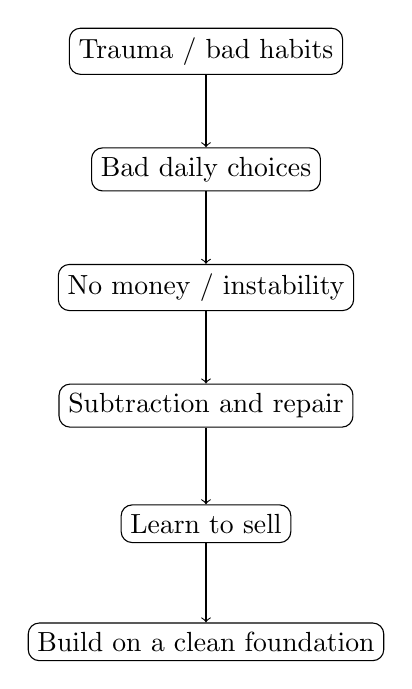
\begin{tikzpicture}
\node[draw, rounded corners] (h) at (0,3) {Trauma / bad habits};
\node[draw, rounded corners] (d) at (0,1.5) {Bad daily choices};
\node[draw, rounded corners] (n) at (0,0) {No money / instability};
\node[draw, rounded corners] (r) at (0,-1.5) {Subtraction and repair};
\node[draw, rounded corners] (s) at (0,-3) {Learn to sell};
\node[draw, rounded corners] (f) at (0,-4.5) {Build on a clean foundation};

\draw[->] (h) -- (d);
\draw[->] (d) -- (n);
\draw[->] (n) -- (r);
\draw[->] (r) -- (s);
\draw[->] (s) -- (f);
\end{tikzpicture}
\caption{A transcript-based reconstruction of the lecture's staged recovery sequence. The order is diagnostic before it is entrepreneurial.}
\end{figure}

This answer is one of the lecture's strongest moments because it is sequential rather than sentimental. We are not told to dream first and repair later. We are told to repair first, then acquire leverage, then build.

\section{Mindset, Skill Set, and the Price of Success}

The lecture now makes explicit a relation that earlier answers had only implied. When asked which matters more, mindset or skill set, the speaker answers: mindset. The reason is selection. A bad mindset does not merely weaken effort. It directs effort into the wrong arena. It makes one copy other people's strategies without first asking what one is actually fitted to do.

\begin{equation}
M \succ S,
\end{equation}
and more precisely,
\begin{equation}
M \Rightarrow \text{choose}(S_{\text{fit}}).
\end{equation}

This is the point at which the lecture retroactively clarifies the earlier claim that a person who has already lost a great deal may still make it back if he retains the right mental and practical architecture. A good mindset does not replace skill. It helps us choose the right one and refuse the wrong one.

The final entrepreneur then gives a blunt piece of financial advice: spend money, but spend it instrumentally. Spend it on information, on network, and on entry into better environments. In the lecture's vocabulary, money is a tool before it is a trophy.

The very last major turn refuses triumphalism. When asked for the deepest life quote he has heard, he answers with ``more money, more problems'' and then explains why. Success changes relationships, expectations, judgment, and the emotional weather of ordinary life. The lecture wants us to preserve this complication. Wealth produces first-order gains, but it also produces second-order burdens.

\begin{equation}
\text{wealth}_{1\text{st order}} \Rightarrow \text{money, access, optionality},
\end{equation}
while
\begin{equation}
\text{wealth}_{2\text{nd order}} \Rightarrow \text{social strain, altered judgment, new burdens}.
\end{equation}

That is the lecture's final widening move. Wealth is neither denied nor romanticized. It is treated as a transformation with a mechanism and a cost. The speaker says, in effect, that success changes not only the bank account but the entire local field of relationships in which the successful person must live.

\section{Summary}

The lecture begins with visible luxury and ends with invisible burden. Between those two poles it constructs a sequence of mechanisms. First, numbers anchor the cases. Then the marketing entrepreneur gives us a theory of production, attention, and visibility. Next, the real-estate developer widens the frame to include timing, values, capital, and fit. Finally, the returning mansion interview turns wealth into diagnosis: bad habits produce bad choices, repair must precede building, mindset chooses skill, and even success must later be paid for in a different currency.

If we compress the chapter into its strongest claims, they are these. Good work without awareness is structurally weak. Advice from the wrong audience is a drag on ambition. Capital is abundant relative to truly investable plans. Financial freedom begins with foundation before it becomes strategy. And the victory, if it comes, does not simplify the world once and for all; it changes the world, and with it the self that enters that world.